\documentclass[12pt,a4paper]{report}

\usepackage[spanish]{babel}
\usepackage[T1]{fontenc}
\usepackage[utf8]{inputenc}
\usepackage{amsmath}
\usepackage{graphicx}
\usepackage[page]{appendix}
\usepackage{listings}
\usepackage{color}
\usepackage{float}
\usepackage{rotating}
\usepackage{graphicx}
\newcommand\scalemath[2]{\scalebox{#1}{\mbox{\ensuremath{\displaystyle #2}}}}

\addto\captionsspanish{\renewcommand\appendixpagename{Archivos de código}}

\DeclareFixedFont{\ttb}{T1}{txtt}{bx}{n}{9}
\DeclareFixedFont{\ttm}{T1}{txtt}{m}{n}{9} 
\DeclareFixedFont{\tti}{T1}{txtt}{m}{it}{9}
\definecolor{comment}{RGB}{150,150,150}

\lstset{
	frame = single, 
	extendedchars=true,	
	showstringspaces=false,
	inputencoding=latin1,
	literate={á}{{\'a}}1 {é}{{\'e}}1 {í}{{\'i}}1 {ó}{{\'o}}1 {ú}{{\'u}}1 {ñ}{{\~n}}1
	{Á}{{\'A}}1 {É}{{\'E}}1 {Í}{{\'I}}1 {Ó}{{\'O}}1 {Ú}{{\'U}}1,
	language=Python,
	basicstyle=\ttm,
	otherkeywords={self},
	keywordstyle=\ttb,
	commentstyle=\tti\color{comment}
	}




% Indica el título del documento como la palabra "Práctica " seguida del número de práctica.
\title{Práctica 2}

% Indica tu nombre completo
\author{Antonio Jesús Heredia Castillo}

\begin{document}

\maketitle

\section*{Ejercicio 1}
En este ejercicio tenemos que implementar una función que resuelva el problema cinemático directo, es decir, que dados los ángulos y la longitud de cada articulación nos devuelva la coordenada $(x,y)$ donde se encuentra el extremo de nuestro robot. Para ello he implementado las formulas:
$$p_x = L_1\cos(\theta_1) + L_2\cos(\theta_1+\theta_2)$$
$$p_y = L_1\sin(\theta_1) + L_2\sin(\theta_1+\theta_2)$$

\section*{Ejercicio 2}
En este ejercicio se nos pide que imprimamos los puntos por los que pasará el extremo de nuestro robot, dados unos puntos.
\begin{lstlisting}[language=Python]
def dibujar_trayectoria_pcd (q1s, q2s , l1 , l2 ):
	xs = []
	ys  = []
	for i,q1 in enumerate(q1s):
		x,y = pcd(q1,q2s[i],l1, l2)
		xs.append(x)
		ys.append(y)
	#Ejercicio 3
	dibujar_robot(q1,q2s[i],l1,l2)
	plt.plot(xs,  ys)
\end{lstlisting}
Como se puede ver en el código lo que realizo es un for sobre los ángulos de $q1s$ y en cada iteración cojo un angulo de $q1s$ y otro de $q2s$, se los paso a la función para calcular la cinemática directa guardando los resultados en un vector para luego mostrarlos todos y que se vea la trayectoria completa. Ademas se puede ver lo que añado para el Ejercicio 3 para que se vea lo que seria el brazo del robot. 
\section*{Ejercicio 4}
En la Figura \ref{fig:ej4} podemos ver el resultado de usar las funciones de los tres ejercicios anteriores.
\begin{figure}[H]
	\centering
	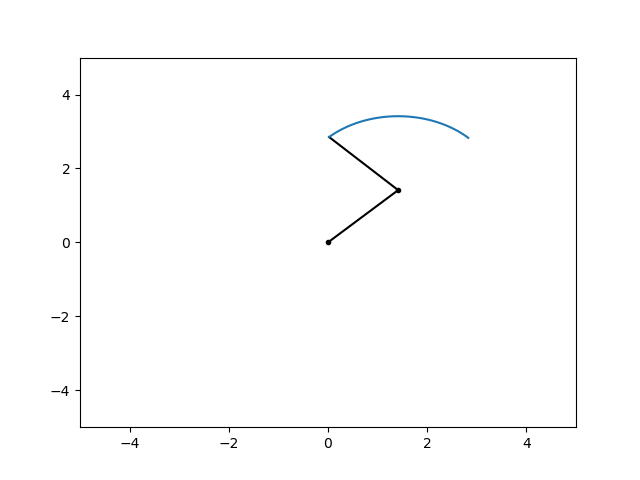
\includegraphics[width=0.7\linewidth]{img/ej4}
	\caption{Trayectoria realizada con las especificaciones del ejercicio 4}
	\label{fig:ej4}
\end{figure}

\section*{Ejercicio 6}
Se puede ver en el ejecutando el código. En la ``animación'' podemos ver como hasta que el primer brazo llega a los $90º$ el segundo brazo aumenta su angulo de forma positiva, una vez que la primera articulación pasa los $90º$ la segunda articulación empieza a decrecer quedando al final la trayectoria de la Figura \ref{fig:ej6}.
\begin{figure}[H]
	\centering
	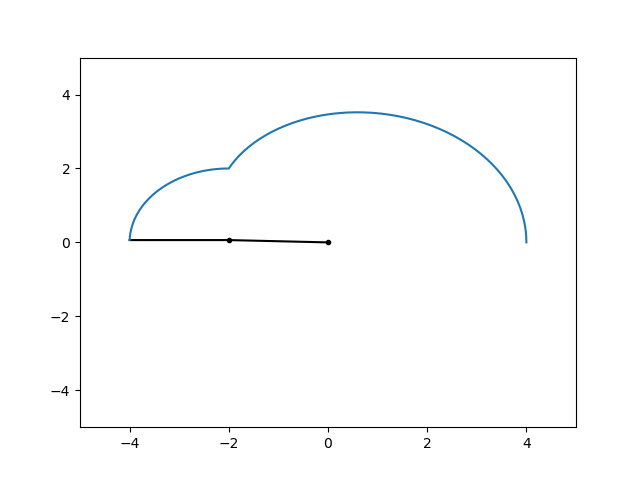
\includegraphics[width=0.7\linewidth]{img/ej6}
	\caption{Trayectoria realizada con las especificaciones del ejercicio 6}
	\label{fig:ej6}
\end{figure}
\section*{Ejercicio  7}
El problema cinemático inverso se resuelve igual de fácil que el directo. Con la cinemática inversa conseguimos los ángulos que tiene que tener nuestras articulaciones para conseguir que el extremo del robot este en un punto determinado.  Para ello hacemos uso de las siguientes ecuaciones:
$$ \cos\theta_2 = \frac{x^2+y^2-L_1^2 -L_2^2}{2L_1 L_2}$$
$$ \tan\theta_1 = \frac{y(L_1 + L_2\cos\theta_2)-xL_2\sin\theta_2}{x(L_1 + L_2\cos\theta_2)+yL_2\sin\theta_2}$$
Como sabemos, en el problema cinemático inverso, la posición en la que se deba encontrar la articulación $i$ depende de la articulación $i+1$ en caso de que esta no sea la ultima. Por eso, el angulo $\theta_1$ depende de $\theta_2$.
\section*{Ejercicio  9}
En este apartado podemos ver el resultado de hacer uso de las funciones implementadas en los dos ejercicios anteriores, para ello haremos pruebas con diferentes listas de puntos. Aunque para ver mas detalles aconsejo ver la animación en el código. \\
Desde el punto $(2,0)$ hasta el punto $(0,2)$:
\begin{figure}[H]
	\centering
	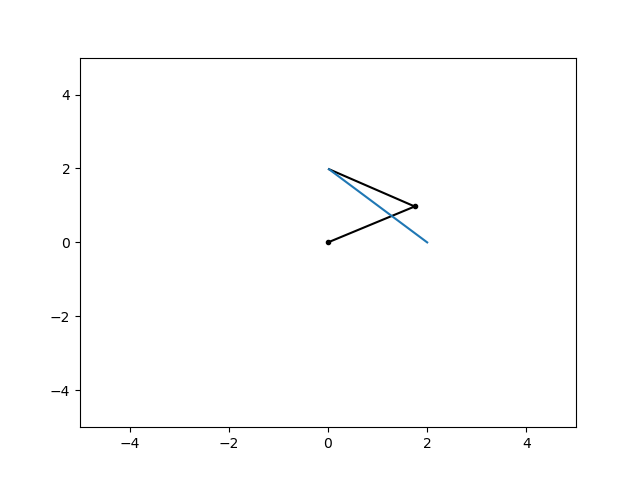
\includegraphics[width=0.7\linewidth]{img/Primer_apartado-Eje_9.png}
	\caption{Desde el punto $(2,0)$ hasta $(0,2)$}
	\label{fig:ej9-a}
\end{figure}
Como podemos ver en la Figura \ref{fig:ej9-a}, en este caso realiza la trayectoria, cosa que no pasara igual en los dos siguientes apartados.\\
Desde el punto $(1,1)$ hasta el punto $(-2,1)$:
\begin{figure}[H]
	\centering
	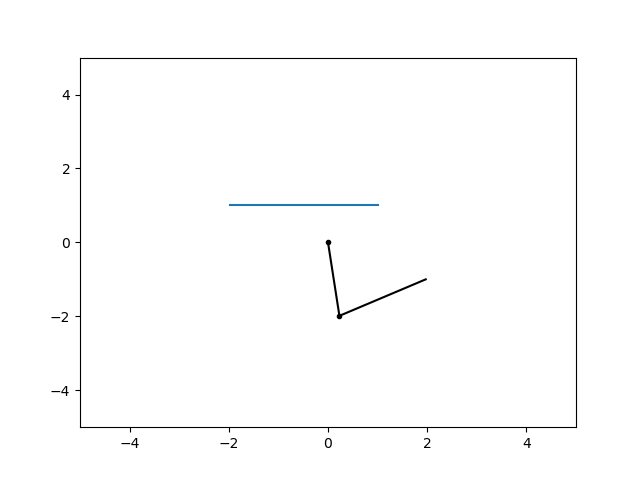
\includegraphics[width=0.7\linewidth]{img/Segundo__apartado-Eje_9.png}
	\caption{Desde el punto $(1,1)$ hasta $(-2,1)$  con arctan}
	\label{fig:ej9-b}
\end{figure}
En la Figura \ref{fig:ej9-b} podemos ver como no acaba bien la simulación y hace cosas raras las articulaciones.  Esto es por que \textbf{arctan} no determina correctamente en que cuadrante se encuentra la solución, creando asi problemas de continuidad. Esto se puede solucionar utilizando \textbf{arctan2}. 
\begin{figure}[H]
	\centering
	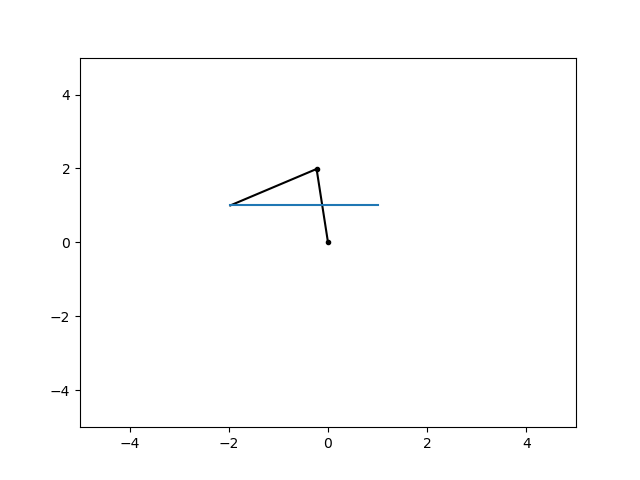
\includegraphics[width=0.7\linewidth]{img/Segundo__apartado-Eje_9-b.png}
	\caption{Desde el punto $(1,1)$ hasta $(-2,1)$  con arctan2}
	\label{fig:ej9-b-b}
\end{figure}
Teniendo al final la solución correcta como podemos ver en la Figura \ref{fig:ej9-b-b}.
\\
Desde el punto $(1,0)$ hasta el punto $(-1,0)$:
\begin{figure}[H]
	\centering
	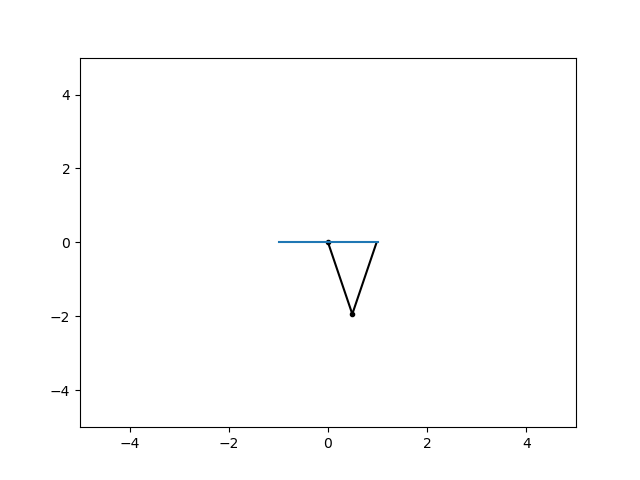
\includegraphics[width=0.7\linewidth]{img/Tercer_apartado-Eje_9.png}
	\caption{Desde el punto $(1,0)$ hasta $(-1,0)$ con arctan}
	\label{fig:ej9-c}
\end{figure}
En la Figura \ref{fig:ej9-c} podemos ver como el extremo del robot empieza acaba en el mismo sitio, en cambio la trayectoria no es esa, esto pasa otra vez por hacer uso de \textbf{arctan}. Lo solucionamos igual que en caso anterior usando \textbf{arctan2}.
\begin{figure}[H]
	\centering
	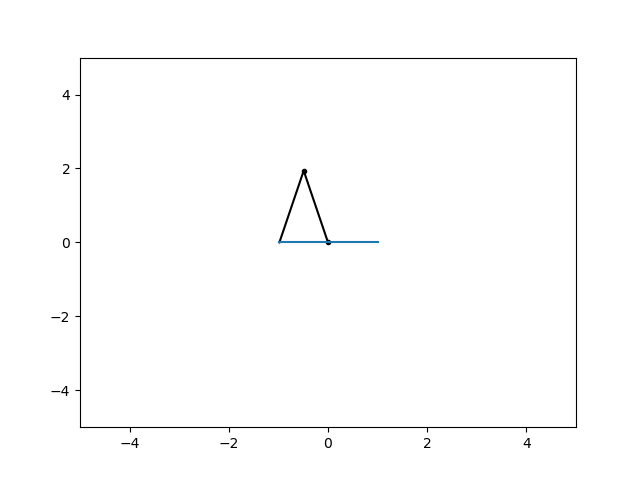
\includegraphics[width=0.7\linewidth]{img/Tercer_apartado-Eje_9-b.png}
	\caption{Desde el punto $(1,0)$ hasta $(-1,0)$ con arctan2}
	\label{fig:ej9-c-b}
\end{figure}
Pero si vemos la animación, volvemos a ver que la articulación se mueve de forma extraña. Cuando $x>0$ la articulación 2 esta en una posición con $y<0$ en cambio cuando $x<0$ la posición de la segunda articulación pasa a ser $y>0$. Esta vez es culpa del \textbf{arccos}, que es el mismo pero en negativo. Este problema lo solucionaremos en el siguiente ejercicio. 
\section*{Ejercicio  10}
En la modificación de este ejercicio conseguiremos que por culpa del coseno, la articulaciones hagan cambio bruscos. Esto lo conseguiremos haciendo que ``el robot'' pueda distinguir cual giro provoca un salto brusco y cual es un giro fluido. Consiguiendo así que se solucione el salto que encontramos en la Figura \ref{fig:ej9-c-b}. En la Figura \ref{fig:ej10-c} podemos ver como ya conseguimos que la articulación 2 siempre tenga una posición de $y<0$. Como siempre esto se podrá ver mejor en la ejecución del código. 
\begin{figure}[H]
	\centering
	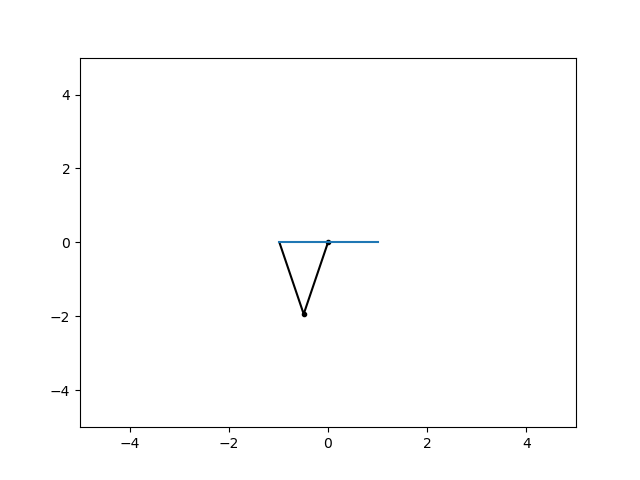
\includegraphics[width=0.7\linewidth]{img/Tercer_apartado-Eje_10.png}
	\caption{Desde el punto $(1,0)$ hasta $(-1,0)$ con arctan2 y viendo cuando hay un cambio brusco.}
	\label{fig:ej10-c}
\end{figure}
\begin{appendices}
	\section*{ejercicio1-2-3-4.py}
	\lstinputlisting{../ejercicio1-2-3-4.py}
	\section*{ejercicio5-6.py}
	\lstinputlisting{../ejercicio5-6.py}
	\section*{ejercicio7-8-9.py}
	\lstinputlisting{../ejercicio7-8-9.py}
	\section*{ejercicio10.py}
	\lstinputlisting{../ejercicio10.py}
\end{appendices}

\end{document}
